%%%%%%%%%%%%%%%%%%%%%%%%%%%%%%%%%%%%%%%%%%%%%%%%%%%%%%%%%%%%%%%%%%%%%%%%%%%%%%%%%
% Template: Exam
%
% Por: Abrantes Araújo Silva Filho
%      abrantesasf@gmail.com
%
% Citação: Se você gostou deste template, por favor ajude a divulgá-lo mantendo
%          o link para meu repositório GitHub em:
%          https://github.com/abrantesasf/LaTeX
%%%%%%%%%%%%%%%%%%%%%%%%%%%%%%%%%%%%%%%%%%%%%%%%%%%%%%%%%%%%%%%%%%%%%%%%%%%%%%%%%




%%%%%%%%%%%%%%%%%%%%%%%%%%%%%%%%%%%%%%%%%%%%%%%%%%%%%%%%%%%%%%%%%%%%%%%%%%%%%%%%%
%%% Configura o tipo de documento, papel, tamanho da fonte e informações básicas
%%% para as proriedades do PDF/DVIPS e outras propriedades do documento
\RequirePackage{ifpdf}
\ifpdf
  % Classe, língua e tamanho da fonte padrão. Outras opções a considerar:
  %   draft
  %   onecolumn (padrão) ou twocolumn (OU usar o package multicol)
  %   fleqn com ou sem leqno (alinhamento à esquerda das fórmulas e dos números)
  %   oneside (padrão para article ou report) ou twoside (padrão para book)
  %   answers = imprime respostas para o gabarito
  \documentclass[pdftex, brazil, 12pt, oneside, addpoints]{exam}
\else
  % Classe, língua e tamanho da fonte padrão. Outras opções a considerar:
  %   draft
  %   onecolumn (padrão) ou twocolumn (OU usar o package multicol)
  %   fleqn com ou sem leqno (alinhamento à esquerda das fórmulas e dos números)
  %   oneside (padrão para article ou report) ou twoside (padrão para book)
  %   answers = imprime respostas para o gabarito
  \documentclass[brazil, 12pt, oneside, addpoints]{exam}
\fi


%%%%%%%%%%%%%%%%%%%%%%%%%%%%%%%%%%%%%%%%%%%%%%%%%%%%%%%%%%%%%%%%%%%%%%%%%%%%%%%%%
%%% Carrega pacotes iniciais necessários para estrutura de controle e para a
%%% criação e o parse de novos comandos
\usepackage{ifthen}
\usepackage{xparse}


%%%%%%%%%%%%%%%%%%%%%%%%%%%%%%%%%%%%%%%%%%%%%%%%%%%%%%%%%%%%%%%%%%%%%%%%%%%%%%%%%
%%% Configuração do tamanho da página, margens, espaçamento entrelinhas e, se
%%% necessário, ativa a indentação dos primeiros parágrafos.
\ifpdf
  \usepackage[pdftex]{geometry}
\else
  \usepackage[dvips]{geometry}
\fi
\geometry{a4paper, left=2.0cm, right=2.0cm, top=2.0cm, bottom=2.0cm}

\usepackage{setspace}
  \singlespacing
  %\onehalfspacing
  %\doublespacing


%%%%%%%%%%%%%%%%%%%%%%%%%%%%%%%%%%%%%%%%%%%%%%%%%%%%%%%%%%%%%%%%%%%%%%%%%%%%%%%%%
%%% Configurações de encoding, lingua e fontes:
\usepackage[T1]{fontenc}
\usepackage[utf8]{inputenc}
\usepackage{babel}

% Altera a fonte padrão do documento (nem todas funcionam em modo math):
%   phv = Helvetica
%   ptm = Times
%   ppl = Palatino
%   pbk = bookman
%   pag = AdobeAvantGarde
%   pnc = Adobe NewCenturySchoolBook
\renewcommand{\familydefault}{ppl}


%%%%%%%%%%%%%%%%%%%%%%%%%%%%%%%%%%%%%%%%%%%%%%%%%%%%%%%%%%%%%%%%%%%%%%%%%%%%%%%%%
%%% Configurações de cabeçalho e rodapé (não pode usar fancyhdr pois ocorre conflito):
\pagestyle{headandfoot}
\runningheadrule
\firstpageheader{}{}{}
\runningheader{Atividade de Recuperação da Aprendizagem}{}{Junho/2019}
\firstpagefooter{}{}{Página \thepage\ de \numpages}
\runningfooter{}{}{Página \thepage\ de \numpages}
\runningfootrule


%%%%%%%%%%%%%%%%%%%%%%%%%%%%%%%%%%%%%%%%%%%%%%%%%%%%%%%%%%%%%%%%%%%%%%%%%%%%%%%%%
%%% Carrega pacotes para referências cruzadas, citações dentro do documento,
%%% links para internet e outros.Configura algumas opções.
%%% Não altere a ordem de carregamento dos packages.
\usepackage{varioref}
\ifpdf
  \usepackage[pdftex]{hyperref}
    \hypersetup{
      % Informações variáveis em cada documento (MUDE AQUI!):
      pdftitle={Atividade de Recuperação da Aprendizagem},
      pdfauthor={Abrantes Araújo Silva Filho},
      pdfsubject={Vetores no plano e no espaço},
      pdfkeywords={vetores, plano, espaço, operações, propriedades},
      pdfinfo={
        CreationDate={}, % Ex.: D:AAAAMMDDHH24MISS
        ModDate={}       % Ex.: D:AAAAMMDDHH24MISS
      },
      % Coisas que você não deve alterar se não souber o que está fazendo:
      unicode=true,
      pdflang={pt-BR},
      bookmarksopen=true,
      bookmarksnumbered=true,
      bookmarksopenlevel=5,
      pdfdisplaydoctitle=true,
      pdfpagemode=UseOutlines,
      pdfstartview=FitH,
      pdfcreator={LaTeX with hyperref package},
      pdfproducer={pdfTeX},
      pdfnewwindow=true,
      colorlinks=true,
      citecolor=green,
      linkcolor=red,
      filecolor=cyan,
      urlcolor=blue
    }
\else
  \usepackage{hyperref}
\fi
\usepackage{cleveref}
\usepackage{url}


%%%%%%%%%%%%%%%%%%%%%%%%%%%%%%%%%%%%%%%%%%%%%%%%%%%%%%%%%%%%%%%%%%%%%%%%%%%%%%%%%
%%% Carrega bibliotecas de símbolos (matemáticos, físicos, etc.), fontes
%%% adicionais, e configura algumas opções
\usepackage{amsmath}
\usepackage{amssymb}
\usepackage{amsfonts}
\usepackage{siunitx}
  \sisetup{group-separator = {.}}
  \sisetup{group-digits = {false}}
  \sisetup{output-decimal-marker = {,}}
\usepackage{bm}
\usepackage{cancel}
% Altera separador decimal via comando, se necessário (prefira o siunitx):
%\mathchardef\period=\mathcode`.
%\DeclareMathSymbol{.}{\mathord}{letters}{"3B}
\usepackage{esvect}
\usepackage{mathtools}
  

%%%%%%%%%%%%%%%%%%%%%%%%%%%%%%%%%%%%%%%%%%%%%%%%%%%%%%%%%%%%%%%%%%%%%%%%%%%%%%%%%
%%% Carrega packages relacionados à computação
\usepackage{algorithm2e}
\usepackage{algorithmicx}
\usepackage{algpseudocode}
\usepackage{listings}
  \lstset{literate=
    {á}{{\'a}}1 {é}{{\'e}}1 {í}{{\'i}}1 {ó}{{\'o}}1 {ú}{{\'u}}1
    {Á}{{\'A}}1 {É}{{\'E}}1 {Í}{{\'I}}1 {Ó}{{\'O}}1 {Ú}{{\'U}}1
    {à}{{\`a}}1 {è}{{\`e}}1 {ì}{{\`i}}1 {ò}{{\`o}}1 {ù}{{\`u}}1
    {À}{{\`A}}1 {È}{{\'E}}1 {Ì}{{\`I}}1 {Ò}{{\`O}}1 {Ù}{{\`U}}1
    {ä}{{\"a}}1 {ë}{{\"e}}1 {ï}{{\"i}}1 {ö}{{\"o}}1 {ü}{{\"u}}1
    {Ä}{{\"A}}1 {Ë}{{\"E}}1 {Ï}{{\"I}}1 {Ö}{{\"O}}1 {Ü}{{\"U}}1
    {â}{{\^a}}1 {ê}{{\^e}}1 {î}{{\^i}}1 {ô}{{\^o}}1 {û}{{\^u}}1
    {Â}{{\^A}}1 {Ê}{{\^E}}1 {Î}{{\^I}}1 {Ô}{{\^O}}1 {Û}{{\^U}}1
    {œ}{{\oe}}1 {Œ}{{\OE}}1 {æ}{{\ae}}1 {Æ}{{\AE}}1 {ß}{{\ss}}1
    {ű}{{\H{u}}}1 {Ű}{{\H{U}}}1 {ő}{{\H{o}}}1 {Ő}{{\H{O}}}1
    {ç}{{\c c}}1 {Ç}{{\c C}}1 {ø}{{\o}}1 {å}{{\r a}}1 {Å}{{\r A}}1
    {€}{{\euro}}1 {£}{{\pounds}}1 {«}{{\guillemotleft}}1
    {»}{{\guillemotright}}1 {ñ}{{\~n}}1 {Ñ}{{\~N}}1 {¿}{{?`}}1
  }
  

%%%%%%%%%%%%%%%%%%%%%%%%%%%%%%%%%%%%%%%%%%%%%%%%%%%%%%%%%%%%%%%%%%%%%%%%%%%%%%%%%
%%% Ativa suporte extendido a cores
\usepackage[svgnames]{xcolor} % Opções de cores: usenames (16), dvipsnames (64),
                              % svgnames (150) e x11names (300).


%%%%%%%%%%%%%%%%%%%%%%%%%%%%%%%%%%%%%%%%%%%%%%%%%%%%%%%%%%%%%%%%%%%%%%%%%%%%%%%%%
%%% Suporte à importação de gráficos externos
\ifpdf
  \usepackage[pdftex]{graphicx}
\else
  \usepackage[dvips]{graphicx}
\fi


%%%%%%%%%%%%%%%%%%%%%%%%%%%%%%%%%%%%%%%%%%%%%%%%%%%%%%%%%%%%%%%%%%%%%%%%%%%%%%%%%
%%% Suporte à criação de gráficos proceduralmente na LaTeX:
\usepackage{tikz}
  \usetikzlibrary{arrows,automata,backgrounds,matrix,patterns,positioning,shapes,shadows}


%%%%%%%%%%%%%%%%%%%%%%%%%%%%%%%%%%%%%%%%%%%%%%%%%%%%%%%%%%%%%%%%%%%%%%%%%%%%%%%%%
%%% Packages para tabelas
\usepackage{array}
\usepackage{longtable}
\usepackage{tabularx}
\usepackage{tabu}
\usepackage{lscape}
\usepackage{colortbl}  
\usepackage{booktabs}
\newcolumntype{M}[1]{>{\centering\arraybackslash}m{#1}}
%\newcolumntype{ML}[1]{>{$}l<{$}}
%\newcolumntype{MR}[1]{>{R}r<{R}}
\newcolumntype{L}[1]{>{\arraybackslash}m{#1}}
\newcolumntype{N}{@{}m{0pt}@{}}


%%%%%%%%%%%%%%%%%%%%%%%%%%%%%%%%%%%%%%%%%%%%%%%%%%%%%%%%%%%%%%%%%%%%%%%%%%%%%%%%%
%%% Packages ambientes de listas
\usepackage{enumitem}
\usepackage[ampersand]{easylist}


%%%%%%%%%%%%%%%%%%%%%%%%%%%%%%%%%%%%%%%%%%%%%%%%%%%%%%%%%%%%%%%%%%%%%%%%%%%%%%%%%
%%% Packages para suporte a ambientes floats, captions, etc.:
\usepackage{float}
\usepackage{wrapfig}
\usepackage{placeins}
\usepackage{caption}
\usepackage{sidecap}
\usepackage{subcaption}


%%%%%%%%%%%%%%%%%%%%%%%%%%%%%%%%%%%%%%%%%%%%%%%%%%%%%%%%%%%%%%%%%%%%%%%%%%%%%%%%%
%%% Meus comandos específicos:
% Commando para ``italizar´´ palavras em inglês (e outras línguas!):
\newcommand{\ingles}[1]{\textit{#1}}

% Commando para colocar o espaço correto entre um número e sua unidade:
\newcommand{\unidade}[2]{\ensuremath{#1\,\mathrm{#2}}}
\newcommand{\unidado}[2]{{#1}\,{#2}}

% Produz ordinal masculino ou feminino dependendo do segundo argumento:
\newcommand{\ordinal}[2]{%
#1%
\ifthenelse{\equal{a}{#2}}%
{\textordfeminine}%
{\textordmasculine}}


%%%%%%%%%%%%%%%%%%%%%%%%%%%%%%%%%%%%%%%%%%%%%%%%%%%%%%%%%%%%%%%%%%%%%%%%%%%%%%%%%
%%% Hifenização específica quando o LaTeX/Babel não conseguirem hifenizar:
\babelhyphenation{Git-Hub}


%%%%%%%%%%%%%%%%%%%%%%%%%%%%%%%%%%%%%%%%%%%%%%%%%%%%%%%%%%%%%%%%%%%%%%%%%%%%%%%%%
%%% Comandos específicos para a classe EXAM deste documento:
\newcommand{\umalinha}{\fillwithlines{0.25in}}
\newcommand{\duaslinhas}{\fillwithlines{0.50in}}
\newcommand{\treslinhas}{\fillwithlines{0.75in}}
\newcommand{\quatrolinhas}{\fillwithlines{1.00in}}
\newcommand{\cincolinhas}{\fillwithlines{1.25in}}
\newcommand{\seislinhas}{\fillwithlines{1.50in}}
\newcommand{\setelinhas}{\fillwithlines{1.75in}}
\newcommand{\oitolinhas}{\fillwithlines{2.00in}}
\newcommand{\novelinhas}{\fillwithlines{2.25in}}
\newcommand{\dezlinhas}{\fillwithlines{2.50in}}

% Verdadeiro ou Falvo para a classe EXAM
\newcommand{\vf}[1][{}]{%
  \fillin[#1][0.25in]%
}

% Título das respostas:
%\renewcommand{\solutiontitle}{\noindent\textbf{Resposta:}\par\noindent}
\renewcommand{\solutiontitle}{\noindent}
%\shadedsolutions
%\SolutionEmphasis{\itshape}

% Comandos para vetores
\newcommand{\vetor}[1]{\ensuremath{\vv{#1}}}
\newcommand{\vetori}{\ensuremath{\hat{i}}}
\newcommand{\vetorj}{\ensuremath{\hat{j}}}
\newcommand{\vetork}{\ensuremath{\hat{k}}}
\newcommand{\norma}[2]{\ensuremath{||\vetor{#2}||_{#1}}}
% normas:
% https://tex.stackexchange.com/a/297263/114611
\let\oldnorm\norm   % <-- Store original \norm as \oldnorm
\let\norm\undefined % <-- "Undefine" \norm
\DeclarePairedDelimiter\norm{\lVert}{\rVert}
% dot product:
%https://tex.stackexchange.com/a/235120/114611
\makeatletter
\newcommand*\bigcdot{\mathpalette\bigcdot@{.5}}
\newcommand*\bigcdot@[2]{\mathbin{\vcenter{\hbox{\scalebox{#2}{$\m@th#1\bullet$}}}}}
\makeatother
% parallel:
%\newcommand{\parallelsum}{\mathbin{\!/\mkern-5mu/\!}}
\newcommand{\paralelo}{\mathbin{\!/\mkern-5mu/\!}}


%%%%%%%%%%%%%%%%%%%%%%%%%%%%%%%%%%%%%%%%%%%%%%%%%%%%%%%%%%%%%%%%%%%%%%%%%%%%%%%%%
%%%%%%%%%%%%%%%%%%%%%%%%%%%%%%%%%%%%%%%%%%%%%%%%%%%%%%%%%%%%%%%%%%%%%%%%%%%%%%%%%
%%%%%%%%%%%%%%%%%%%%%%%%%%%%%%%%%%%%%%%%%%%%%%%%%%%%%%%%%%%%%%%%%%%%%%%%%%%%%%%%%
%%%%%%%%%%%%%%%%%%%%%%%%%%%%%%%%%%%%%%%%%%%%%%%%%%%%%%%%%%%%%%%%%%%%%%%%%%%%%%%%%
%%%%%%%%%%%%%%%%%%%%%%%%%%%%%% COMEÇA O DOCUMENTO %%%%%%%%%%%%%%%%%%%%%%%%%%%%%%%
%%%%%%%%%%%%%%%%%%%%%%%%%%%%%%%%%%%%%%%%%%%%%%%%%%%%%%%%%%%%%%%%%%%%%%%%%%%%%%%%%
%%%%%%%%%%%%%%%%%%%%%%%%%%%%%%%%%%%%%%%%%%%%%%%%%%%%%%%%%%%%%%%%%%%%%%%%%%%%%%%%%
%%%%%%%%%%%%%%%%%%%%%%%%%%%%%%%%%%%%%%%%%%%%%%%%%%%%%%%%%%%%%%%%%%%%%%%%%%%%%%%%%
%%%%%%%%%%%%%%%%%%%%%%%%%%%%%%%%%%%%%%%%%%%%%%%%%%%%%%%%%%%%%%%%%%%%%%%%%%%%%%%%%
\begin{document}


%%%%%%%%%%%%%%%%%%%%%%%%%%%%%%%%%%%%%%%%%%%%%%%%%%%%%%%%%%%%%%%%%%%%%%%%%%%%%%%%%
%%%%%%%%%%%%%%%%%%%%%%%%%%%%%%%%%%%%%%%%%%%%%%%%%%%%%%%%%%%%%%%%%%%%%%%%%%%%%%%%%
%%%%%%%%%%%%%%%%%%%%%%%%%%%%%%%%%%%%%%%%%%%%%%%%%%%%%%%%%%%%%%%%%%%%%%%%%%%%%%%%%
\begin{coverpages}

\begin{center}
\textbf{\textit{\Large%
Álgebra Linear e Geometria Analítica}}
\end{center}

\vspace{1cm}

\begin{figure}[H]
\begin{center}
\fbox{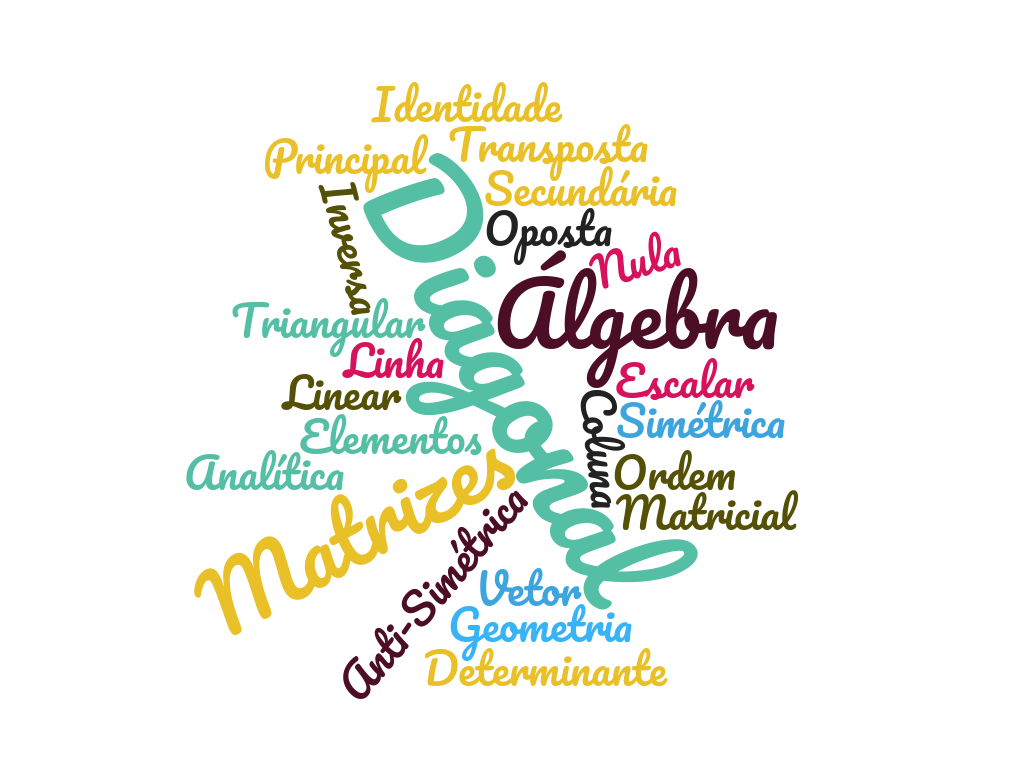
\includegraphics[scale=0.4]{linear_algebra.png}}
\end{center}
\end{figure}

\vspace{1cm}

\begin{center}
\textit{\textbf{\Large%
    --- Atividade de Recuperação da Aprendizagem ---\\%
\ \\%
    Vetores no Plano e no Espaço\\%
\ \\%
Junho/2019}}
\end{center}

%\vspace{1cm}
%\begin{flushright}
%\textbf{Monitor(es):}\\
%\textit{Monitor 1\\
%Monitor 2}
%\end{flushright}

%\begin{center}
%  \fbox{\fbox{\parbox{5.5in}{\centering
%        Answer the questions in the spaces provided on the
%        question sheets. If you run out of room for an answer,
%        continue on the back of the page.}}}
%\end{center}

\end{coverpages}

\newpage


%%%%%%%%%%%%%%%%%%%%%%%%%%%%%%%%%%%%%%%%%%%%%%%%%%%%%%%%%%%%%%%%%%%%%%%%%%%%%%%%%
%%%%%%%%%%%%%%%%%%%%%%%%%%%%%%%%%%%%%%%%%%%%%%%%%%%%%%%%%%%%%%%%%%%%%%%%%%%%%%%%%
%%%%%%%%%%%%%%%%%%%%%%%%%%%%%%%%%%%%%%%%%%%%%%%%%%%%%%%%%%%%%%%%%%%%%%%%%%%%%%%%%
\makebox[15cm]{Nome:\enspace\hrulefill}

\vspace{0.5cm}

\makebox[15cm]{Curso:\enspace\hrulefill}

\fullwidth{\section{Instruções importantes}}

Esta \emph{Atividade de Recuperação da Aprendizagem} consiste de
67 questões, das quais 18 são obrigatórias\footnote{DICA IMPORTANTE:
  não se limite a fazer as questões obrigatórias, pelo menos \emph{leia} as
  outras questões para identificar conteúdos que você ainda não
  domina! Se, ao ler as questões opcionais, você perceber que não
  domina o conteúdo, faça essas questões também! Assim você terá o
  máximo aproveitamente desta atividade.}, que abordam o seguinte conteúdo:

\begin{itemize}
\item Vetores no plano e no espaço
  \begin{itemize}
  \item Conceitos básicos
  \item Representação e propriedades de vetores
  \item Operações no plano
  \item Operações no espaço
  \end{itemize}
\end{itemize}

\begin{center}
  \fbox{\parbox{10cm}{\begin{center}\textbf{QUESTÕES OBRIGATÓRIAS:}

        \emph{1, 5, 12, 13, 19, 20, 28, 30, 32,\\ 37, 38,
          39, 43, 46, 55, 56, 62 e 63}.

        \vspace{0.5cm}
    \textbf{PRAZO PARA ENTREGA: DIA 12/06/2019}!
    \end{center}}}
\end{center}

As regras abaixo devem ser obedecidas:

\begin{enumerate}
  \item A atividade poderá ser feita durantes as monitorias ou
        como atividade para casa;
  \item O monitor não dará respostas, mas explicará a matéria e
        esclarecerá dúvidas tantas vezes quanto necessário;
  \item As respostas serão escritas em folhas de papel almaço,
        disponibilizadas pelo monitor. Não se esqueça de escrever seu
        nome nas folhas;
  \item As questões de verdadeiro ou falso (V ou F) e/ou questões
        objetivas podem ser resolvidas na própria folha de
        questões. Questões discursivas devem ser resolvidas na própria
        folha ou na folha de papel almaço;
  \item É permitido a consulta de qualquer material bibliográfico,
        impresso ou online, e também é permitido o uso de calculadoras
        (desde que o desenvolvimento de todas as contas esteja
        descrito);
  \item Essa atividade servirá para recuperar, além da aprendizagem,
        uma parte da nota da segunda avaliação. As regras para isso
        ainda serão definidas pelo Prof. Rober. Observação: recuperar
        a nota é a conseqüência, o objetivo é recuperar a aprendizagem!
\end{enumerate}


\newpage
\begin{questions}
\setlength\linefillthickness{0.2pt}
%%%%%%%%%%%%%%%%%%%%%%%%%%%%%%%%%%%%%%%%%%%%%%%%%%%%%%%%%%%%%%%%%%%%%%%%%%%%%%%%%
%%%%%%%%%%%%%%%%%%%%%%%%%%%%%%%%%%%%%%%%%%%%%%%%%%%%%%%%%%%%%%%%%%%%%%%%%%%%%%%%%
%%%%%%%%%%%%%%%%%%%%%%%%%%%%%%%%%%%%%%%%%%%%%%%%%%%%%%%%%%%%%%%%%%%%%%%%%%%%%%%%%
\fullwidth{\section{Vetores: conceitos fundamentais}}

\question
O que é um vetor? O que diferencia um vetor de um escalar?
\quatrolinhas

\question
Identifique abaixo se a grandeza indicada é vetorial (V) ou escalar (E):
\begin{parts}
  \part \vf[E] Massa de uma pessoa, em kg.
  \part \vf[V] Deslocamento, em km, de uma pessoa, de um ponto A para o ponto B.
  \part \vf[E] Altura de uma pessoa, em m.
  \part \vf[V] Peso de uma pessoa, em N\footnote{N é o símbolo do
    \textbf{newton}, uma unidade de medida de força:
    $\displaystyle 1N = 1 \frac{kg \times m}{s^2}$}.
  \part \vf[V] A direção de uma avião, voando de Vitória para São
  Paulo.
  \part \vf[E] O Índice de Massa Corporal (IMC) de uma pessoa, calculado
  como $\displaystyle IMC = \frac{m}{a^2}$, onde $m$ é massa em kg, e  $a$ é a altura em m.
\end{parts}

\question
Os vetores podem ser representados de \emph{muitas} formas diferentes
(e isso causa até uma certa confusão para quem está começando a
estudar o assunto). Considere que temos um vetor \vetor{u} qualquer em
$\mathbb{R}^2$,
que \textbf{sai} do ponto A e \textbf{chega} no ponto B em um sistema de coordenadas.
Assinale abaixo todas as formas corretas de se representar esse vetor.
\begin{checkboxes}
  \choice \vetor{AB}
  \choice \vetor{u}
  \choice $u = AB$
  \choice \vetor{BA}
  \choice $\vetor{u} = x\vetori + y\vetorj$
  \choice $\vetor{u} = u_x\vetori + u_y\vetorj$
\end{checkboxes}

\question
O \emph{comprimento} de um vetor também pode ser representado por
diversas denominações (mais uma fonte de confusão!). Assinale abaixo
todas as formas corretas de se denominar o comprimento de um vetor
\vetor{u} qualquer.
\begin{checkboxes}
  \choice tamanho
  \choice magnitude
  \choice norma
  \choice módulo
  \choice valor absoluto
  \choice $\lVert \vetor{u} \rVert$
  \choice $u$
  \choice $|\vetor{u}|$
\end{checkboxes}

\question
O que significa a \emph{direção} de um vetor? E o \emph{sentido}?
\cincolinhas

\question
Assinale a (única) alternativa verdadeira:
\begin{checkboxes}
  \choice Dois vetores são iguais se tiverem a mesma magnitude, não
  importando a direção ou o sentido.
  \choice A magnitude de um vetor pode ser 0, um valor positivo, ou um
  valor negativo.
  \choice Dois vetores com a mesma magnitude, direção e sentido, mas
  localizados em locais diferentes no espação, são diferentes.
  \choice Dois vetores com a mesma magnitude, mesma direção, mas
  sentidos opostos são iguais.
  \choice Dois vetores são iguais se, e somente se, tiverem a mesma
  magnitude, direção e sentido, mesmo que estejam em locais diferentes
  no espaço.
  \choice Dois vetores são iguais se, e somente se, forem colineares.
  \choice Não existem vetores nulos.
\end{checkboxes}

\question
Se a magnitude de dois vetores for a mesma, $\lVert \vetor{a} \rVert =
\lVert \vetor{b} \rVert$, então podemos afirmar que os vetores serão
iguais? Justifique sua resposta.
\treslinhas

\question
Assinale verdadeiro (V) ou falso (F):
\begin{parts}
  \part \vf[] $\vetor{v} + \vetor{0} = \vetor{v}$
  \part \vf[] $\vetor{v} + (- \vetor{v}) = \vetor{0}$
  \part \vf[] $\vetor{v} - \vetor{w} = \vetor{v} + (- \vetor{w})$
  \part \vf[] $\vetor{v} + \vetor{w} \ne \vetor{w} + \vetor{v}$
\end{parts}

\question
Quando ``escalonamos'' um vetor \vetor{v} qualquer através da
multiplicação desse vetor com um número escalar $k$ qualquer, o
resultado será um \emph{múltiplo escalar} de \vetor{v}. Assinale
verdadeiro (V) ou falso (F):
\begin{parts}
  \part \vf[] Se $\vetor{w} = k\vetor{v}$, então $\lVert \vetor{w}
  \rVert =
  |k|\lVert \vetor{v} \rVert$
  \part \vf[] Se $\vetor{w} = k\vetor{v}$, então \vetor{w} será nulo
  se, e apenas se, $k$ for igual a zero ou \vetor{v} for igual ao
  vetor nulo.
  \part \vf[] Se $\vetor{w} = k\vetor{v}$, então \vetor{w} pode ser
  paralelo ou perpendicular a \vetor{v}.
  \part \vf[] Se $\vetor{w} = k\vetor{v}$, então \vetor{w} sempre terá
  a mesma direção de \vetor{v}.
  \part \vf[] Se $\vetor{w} = k\vetor{v}$, então \vetor{w} sempre terá
  o mesmo sentido de \vetor{v}.
  \part \vf[] É possível obter um vetor \vetor{w} de magnitude 1
  multiplicando-se um vetor \vetor{v} pelo inverso de sua magnitude,
  ou seja, $\displaystyle \vetor{w} = \frac{1}{\lVert \vetor{v}
    \rVert} \vetor{v}$. Esse vetor \vetor{w}, além de ter magnitude 1,
  também terá o mesmo sentido e direção do vetor \vetor{v}.
\end{parts}


%%%%%%%%%%%%%%%%%%%%%%%%%%%%%%%%%%%%%%%%%%%%%%%%%%%%%%%%%%%%%%%%%%%%%%%%%%%%%%%%%
%%%%%%%%%%%%%%%%%%%%%%%%%%%%%%%%%%%%%%%%%%%%%%%%%%%%%%%%%%%%%%%%%%%%%%%%%%%%%%%%%
%%%%%%%%%%%%%%%%%%%%%%%%%%%%%%%%%%%%%%%%%%%%%%%%%%%%%%%%%%%%%%%%%%%%%%%%%%%%%%%%%
\fullwidth{\section{Componentes e Vetores Componentes}}

\question
A figura abaixo ilustra o \emph{vetor} \vetor{A} juntamente com seus
\emph{vetores componentes} \vetor{A_x} e \vetor{A_y}.
\begin{figure}[H]
  \begin{center}
    \fbox{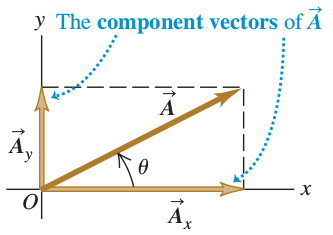
\includegraphics[scale=0.6]{vetor1.png}}\\
    \footnotesize{Fonte:~Young HD, Freedman RA, Ford
      LA. \emph{University Physics}, 13.\ ed.}
  \end{center}
\end{figure}
\vspace{-0.7cm}
\begin{parts}
  \part Qual a diferença, e a relação, entre um determinado
  \textbf{vetor} \vetor{A} e seus \emph{\textbf{vetores componentes}} \vetor{A_x} e \vetor{A_y}?
  \quatrolinhas
  \part Como representar um vetor \vetor{A} em termos de seus
  \emph{vetores componentes} \vetor{A_x} e \vetor{A_y}?
  \umalinha
\end{parts}

\question
A figura abaixo ilustra o \emph{vetor} \vetor{A} juntamente com seus
\emph{componentes} $A_x$ e $A_y$.
\begin{figure}[H]
  \begin{center}
    \fbox{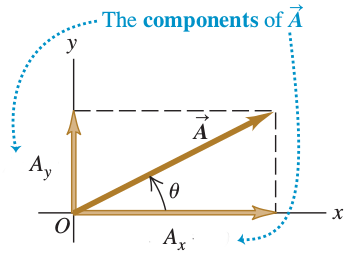
\includegraphics[scale=0.6]{vetor2b.png}}\\
    \footnotesize{Fonte:~Young HD, Freedman RA, Ford
      LA. \emph{University Physics}, 13.\ ed.}
  \end{center}
\end{figure}
\vspace{-0.7cm}
\begin{parts}
  \part O que é um \emph{\textbf{componente}} de um vetor? (não
  cofunda com ``vetor componente'')
  \treslinhas
  \part Como representar um vetor \vetor{A} em termos de seus
  \emph{componentes} $A_x$ e $A_y$?
  \umalinha
  \part Os \emph{componentes} $A_x$ e $A_y$ são vetores? Por quê? (de novo, não
  confunda ``componente'' com ``vetor componente'')
  \duaslinhas
\end{parts}

\question
Um vetor \vetor{w} em $\mathbb{R}^2$ sai do ponto $P = (-4, 5)$ e
chega no ponto $Q = (3, -12)$. Que vetor é esse? (represente esse vetor
em termos de seus \emph{componentes})

\question
Um vetor \vetor{u} em $\mathbb{R}^5$ sai do ponto $P = (3, 4, -2, 1,
-8)$ e chega no ponto $Q = (-1, -1, 4, 8, 2)$. Que vetor é esse?
(represente esse vetor em termos de seus \emph{componentes})

\question
Considere a figura abaixo, que representa um vetor \vetor{V} no espaço
em três dimensões, e responda verdadeiro (V) ou falso (F):
\begin{figure}[H]
  \begin{center}
    \fbox{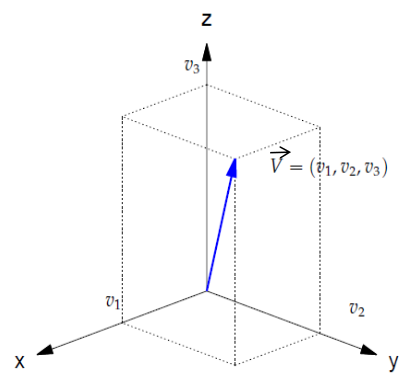
\includegraphics[scale=0.5]{vetor3.png}}\\
    \footnotesize{Fonte:~slides do material da disciplina}
  \end{center}
\end{figure}
\vspace{-0.7cm}
\begin{parts}
  \part \vf[] $v_1$, $v_2$ e $v_3$ representam os vetores
  componentes de \vetor{V}.
  \part \vf[] Podemos considerar que $(v_1$, $v_2$, $v_3)$ são as
  coordenadas $(x, y, z)$ do ponto final de \vetor{V}, já que esse vetor se inicia
  na origem do sistema cartesiano.
  \part \vf[] $\vetor{V} = (v_1$, $v_2$, $v_3)$ é a representação do
  vetor \vetor{V} através de seus componentes.
  \part \vf[] Uma outra forma de representar o vetor \vetor{V} seria
  através dos vetores componentes, da seguinte forma: $\vetor{V} =
  \vetor{v_1} + \vetor{v_2} + \vetor{v_3}$.
  \part \vf[] Podemos usar os componentes para representar o vetor
  \vetor{V} da seguinte forma: $\vetor{V} = v_1\,\vetori + v_2\,\vetorj + v_3\,\vetork$.
\end{parts}

\question
Eu entendi a diferença entre ``componente'' e ``vetor componente'',
bem como as formas de representar um vetor utilizando componentes ou
utilizando vetors componentes!
\begin{checkboxes}
  \choice Sim
  \choice Não
\end{checkboxes}


%%%%%%%%%%%%%%%%%%%%%%%%%%%%%%%%%%%%%%%%%%%%%%%%%%%%%%%%%%%%%%%%%%%%%%%%%%%%%%%%%
%%%%%%%%%%%%%%%%%%%%%%%%%%%%%%%%%%%%%%%%%%%%%%%%%%%%%%%%%%%%%%%%%%%%%%%%%%%%%%%%%
%%%%%%%%%%%%%%%%%%%%%%%%%%%%%%%%%%%%%%%%%%%%%%%%%%%%%%%%%%%%%%%%%%%%%%%%%%%%%%%%%
\fullwidth{\section{Soma, subtração, múltiplos escalares e magnitude
    de vetores}}

\question
Dados os pontos $A = (-2, 6)$, $B = (4, 10)$, $C = (6, -2)$ e $O = (0,
0)$, calcule:
\begin{parts}
  \part $\vetor{OA} - \vetor{AB}$
  \part $\vetor{OC} - \vetor{BC}$
  \part $3\,\vetor{BA} - 4\,\vetor{CB}$
  \part $\vetor{OO} - \vetor{AC}$
\end{parts}

\question
Seja o vetor $\vetor{u} = (-1, 3)$. Sabendo-se que esse vetor termina
no ponto $Q = (3, 1)$, qual é seu ponto de origem $P$?

\question
Dados os vetores $\vetor{v} = (3, -1)$ e $\vetor{u} = (-1, 2)$, ache o
vetor \vetor{x} tal que:
\begin{parts}
  \part $\displaystyle 4\,(\vetor{v}-\vetor{u})+\frac{1}{3}\,\vetor{x} =
  2\,\vetor{v} - \vetor{x}$
  \part $\displaystyle 3\,\vetor{x}-(2\,\vetor{u}-\vetor{v}) =
  2\,(4\,\vetor{x}-3\,\vetor{v})$
\end{parts}

\question
Dados os vetores $\vetor{u} = (6, -2)$, $\vetor{v} = (-6, 8)$ e
$\vetor{w} = (4, -3)$:
\begin{parts}
  \part Calcule $\lVert \vetor{u} \rVert$.
  \part Encontre o \emph{vetor unitário} de sentido oposto ao vetor
  \vetor{w}.
  \part Encontre um vetor que tenha a metade do tamanho de \vetor{v},
  tenha a mesma direção, mas sentido contrário.
  \part Qual o tamanho do vetor que é resultante da soma do dobro do
  vetor \vetor{u} com a metade do vetor \vetor{w}?
  \part Qual o resultado de $\displaystyle
  \left\lVert\frac{\vetor{w}}{\lVert \vetor{w} \rVert}\right\rVert$?
\end{parts}

\question
Dadas as coordenadas $(2, -6, z)$ de um vetor \vetor{x} em
$\mathbb{R}^3$, encontre o valor da coordenada $z$ de maneira que
$\lVert \vetor{x} \rVert = 15$.

\question
Qual a norma do vetor $\vetor{a} \in \mathbb{R}^7 = (2, 3, -1, 0, 4,
-1, 5)$?

\question
É possível somar ou subtrair o vetor $\vetor{r} \in \mathbb{R}^4$ com
o vetor $\vetor{s} \in \mathbb{R}^5$? Justifique sua resposta.
\duaslinhas

\question
Quanto vale a metade da norma do vetor $\vetor{b} = -2\,\vetori +
3\,\vetorj - 5\,\vetork$?

\question
Eu entendi como calcular a soma e subtração de vetores. Também entendi
como encontrar um vetor unitário e um múltiplo escalar de qualquer
vetor. Por fim, já entendi e sei calcular o que é a norma de um vetor.
\begin{checkboxes}
  \choice Sim
  \choice Não
\end{checkboxes}


%%%%%%%%%%%%%%%%%%%%%%%%%%%%%%%%%%%%%%%%%%%%%%%%%%%%%%%%%%%%%%%%%%%%%%%%%%%%%%%%%
%%%%%%%%%%%%%%%%%%%%%%%%%%%%%%%%%%%%%%%%%%%%%%%%%%%%%%%%%%%%%%%%%%%%%%%%%%%%%%%%%
%%%%%%%%%%%%%%%%%%%%%%%%%%%%%%%%%%%%%%%%%%%%%%%%%%%%%%%%%%%%%%%%%%%%%%%%%%%%%%%%%
\fullwidth{\section{Produto escalar entre dois vetores}}

\question
Sejam 2 vetores, \vetor{u} e \vetor{w}. O produto escalar entre esses
dois vetores resulta em um valor escalar, e é simbolizado por $\vetor{u} \bigcdot \vetor{w}$.
Existem duas maneiras de se calcular o produto escalar entre esses
dois vetores: a) através de seus componentes; e b) através das magnitudes e
do ângulo entre eles. Pergunta-se: 
\begin{parts}
  \part Como calcular o produto escalar através dos componentes dos
  vetores?
  \treslinhas
  \part Se soubermos qual o ângulo entre esses vetores e se soubermos
  qual a magnitude de cada um, como calcular o produto escalar entre
  eles?
  \treslinhas
\end{parts}

\question
Sabe-se que $\lVert \vetor{x} \rVert = 8$ e que $\lVert \vetor{y}
\rVert = 4$. Sabe-se também que o ângulo entre esses dois vetores é de
60º. É possível calcular $\vetor{x} \bigcdot \vetor{y}$\,? Se sim, calcule.

\question
Calcule o produto escalar entre os vetores $\vetor{a} = (1, 2, 3, 4,
5)$ e $\vetor{b} = (5, 4, 3, 2, 1)$.

\question
Sabendo-se que $\vetor{r} \bigcdot \vetor{s} = -15$, $\lVert
\vetor{r} \rVert = \sqrt{26}$ e $\lVert \vetor{s} \rVert = \sqrt{41}$,
calcule o ângulo $\theta$ entre esses vetores. Antes de calcular o ângulo, você
anteciparia que: a) $0º \le \theta < 90º$; ou b) $\theta = 90º$; ou c)
$90º < \theta \le 180º$? Calcule e confira.

\question
Calcule o ângulo entre o vetor $\vetor{w} = 3\,\vetori - 2\,\vetorj$ e
o vetor $\vetor{z} = 5\,\vetori + 1\,\vetorj$.

\question
Sendo $\vetor{a} = (2, -1, 1)$, $\vetor{b} = (1, -2, -2)$ e $\vetor{c}
= (1, 1, -1)$, encontre o vetor $\vetor{x} = (x, y, z)$ tal que:
$\vetor{v} \bigcdot \vetor{a} = 4$; $\vetor{v} \bigcdot \vetor{b} = -9$;
e $\vetor{v} \bigcdot \vetor{c} = 5$.

\question
Responda verdadeiro (V) ou falso (F):
\begin{parts}
  \part \vf[] Se dois vetores são ortogonais entre si, não é possível
  calcular o produto escalar.
  \part \vf[] Podemos afirmar com certza que: se o produto escalar
  entre dois vetores é negativo, então o ângulo entre eles será maior
  do que 90º e menor ou igual a 180º.
  \part \vf[] O produto escalar entre dois vetores será nulo se: um
  deles for um vetor nulo, ou o ângulo entre eles for de 90º
  \part \vf[] Se só temos a informação sobre os componentes de dois
  vetores, podemos calcular o produto escalar entre eles, mas não o
  ângulo.
  \part \vf[] Dependendo da situação, o produto escalar entre dois
  vetores pode resultar em um outro vetor.
  \part \vf[] O produto escalar entre dois vetores nunca será nulo.
\end{parts}

\question
Determinar o valor de $x$ para que os vetores $\vetor{v} = x\,\vetori
- 2\,\vetorj + 3\,\vetork$\ e $\vetor{w} = 2\,\vetori - \vetorj +
2\,\vetork$ sejam ortogonais.

\question
Eu entendi como calcular o produto escalar entre dois vetores, tanto
usando os componentes, quanto usando as magnitudes e o ângulo entre eles.
\begin{checkboxes}
  \choice Sim
  \choice Não
\end{checkboxes}

\question
Uma última questão para saber se você realmente entendeu o produto
escalar: determine o ângulo entre a diagonal de um cubo unitário e a
aresta no eixo $x$, conforme a figura abaixo:
\begin{figure}[H]
  \begin{center}
    \fbox{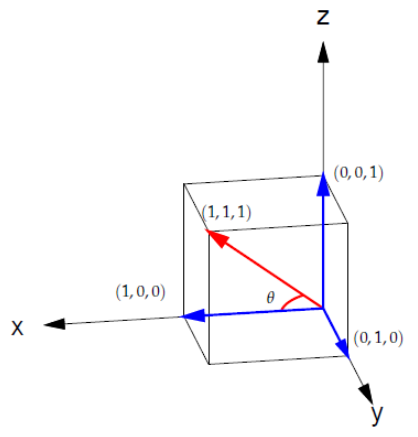
\includegraphics[scale=0.4]{vetor4.png}}\\
    \footnotesize{Fonte:~slides do material da disciplina}
  \end{center}
\end{figure}



%%%%%%%%%%%%%%%%%%%%%%%%%%%%%%%%%%%%%%%%%%%%%%%%%%%%%%%%%%%%%%%%%%%%%%%%%%%%%%%%%
%%%%%%%%%%%%%%%%%%%%%%%%%%%%%%%%%%%%%%%%%%%%%%%%%%%%%%%%%%%%%%%%%%%%%%%%%%%%%%%%%
%%%%%%%%%%%%%%%%%%%%%%%%%%%%%%%%%%%%%%%%%%%%%%%%%%%%%%%%%%%%%%%%%%%%%%%%%%%%%%%%%
\fullwidth{\section{Decomposição de um vetor em componentes}}

\question
O que é decompor um vetor em seus componentes?
\quatrolinhas

\question
Imagine que temos o vetor $\vetor{a} \in \mathbb{R}^2$. Sabemos 
a magnitude desse vetor e o ângulo $\theta$ que esse vetor faz com o
eixo $x$ no plano cartesiano.
\begin{parts}
\part Qual das fórmulas
abaixo nos fornecerá o componente vertical do \vetor{a}?
\begin{checkboxes}
  \choice $\displaystyle a_y = \lVert \vetor{a}
  \rVert \cos{(\theta)}$
  \choice $\displaystyle a_y = \lVert \vetor{a}
  \rVert \sin{(\theta)}$
\end{checkboxes}
\part Qual das fórmulas
abaixo nos fornecerá o componente horizontal do \vetor{a}?
\begin{checkboxes}
  \choice $\displaystyle a_x = \lVert \vetor{a}
  \rVert \cos{(\theta)}$
  \choice $\displaystyle a_x = \lVert \vetor{a}
  \rVert \sin{(\theta)}$
\end{checkboxes}
\part Responda verdadeiro (V) ou falso (F):
\begin{parts}
  \part \vf[] Sempre que soubermos a magnitude de um determinado vetor
  e sua direção, será possível decompor esse vetor em seus
  componentes.
  \part \vf[] Se soubermos a magnitude de um vetor e a magnitude de um
  de apenas 1 de seus componentes, não será possível calcular sua
  direção.
  \part \vf[] A partir dos componentes, podemos encontrar os vetores
  componentes.
  \part \vf[] Se eu conheço a magnitude de um vetor mas não sei sua
  direção, então não é possível determinar seus componentes.
\end{parts}
\end{parts}

\question
Seja $\lVert \vetor{m} \rVert = 5$. Sabendo que \vetor{m} tem direção $-30$º a partir do
eixo $x$ do plano cartesiano.
\begin{parts}
  \part Encontre os componentes $m_x$ e $m_y$.
  \part Escreva o vetor \vetor{m} utilizando seus componentes.
\end{parts}

\question
Sendo $\lVert \vetor{w} \rVert = 5$ e $w_y = 3$,
encontre o ângulo $\theta$ que esse vetor faz com o eixo $x$, ou seja,
encontre sua direção.

\question
Sendo $v_x = 5$, e a direção do vetor \vetor{v}
igual a $\theta = 45$º, encontre o tamanho do vetor \vetor{v}.

\question
Eu entendi como decompor um vetor em seus componentes!
\begin{checkboxes}
  \choice Sim
  \choice Não
\end{checkboxes}


%%%%%%%%%%%%%%%%%%%%%%%%%%%%%%%%%%%%%%%%%%%%%%%%%%%%%%%%%%%%%%%%%%%%%%%%%%%%%%%%%
%%%%%%%%%%%%%%%%%%%%%%%%%%%%%%%%%%%%%%%%%%%%%%%%%%%%%%%%%%%%%%%%%%%%%%%%%%%%%%%%%
%%%%%%%%%%%%%%%%%%%%%%%%%%%%%%%%%%%%%%%%%%%%%%%%%%%%%%%%%%%%%%%%%%%%%%%%%%%%%%%%%
\fullwidth{\section{Projeção ortogonal}}

\question
O que é encontrar a \emph{projeção ortogonal} de um vetor sobre outro?
\quatrolinhas

\question
Imagine que precisamos projetar o vetor \vetor{b} sobre o vetor
\vetor{a}. Sabemos quais são os componentes de cada vetor, mas não
sabemos o ângulo $\theta$ entre eles.
\begin{parts}
  \part Como calcular a projeção de \vetor{b} que é paralela ao vetor
  \vetor{a}?
  \part Como calcular a projeção de \vetor{b} que é ortogonal ao vetor
  \vetor{a}?
\end{parts}

\question
Sejam os vetores $\vetor{v} = (2, -1, 3)$ e $\vetor{w} = (4, -1,
2)$. Encontre os vetores \vetor{r} e \vetor{s} tais que $\vetor{r}
\paralelo \vetor{w}$, e $\vetor{s} \bot \vetor{w}$.

\question
É possível obter a projeção ortogonal de um vetor $\vetor{a} \in
\mathbb{R}^3$ sobre um vetor $\vetor{b} \in \mathbb{R}^4$? Justifique
sua resposta.
\duaslinhas

\question
Sejam dois vetores, \vetor{x} e \vetor{y}. O que estamos obtendo se
utilizarmos a seguinte fórmula:
\begin{equation*}
  \vetor{x} - \text{proj}_{\vetor{y}}\vetor{x} = \vetor{x} -
  \left(\frac{\vetor{x} \bigcdot \vetor{y}}{\lVert \vetor{y} \rVert^2}\right)\vetor{y}
\end{equation*}

\question
Decomponha o vetor $\vetor{v} = (-1, 2, -3)$ em dois vetores \vetor{a}
e \vetor{b}, tais que $\vetor{a} \paralelo \vetor{u}$ e $\vetor{b} \bot
\vetor{u}$, sendo $\vetor{u} = (2, 1, -1)$.

\question
Eu entendi como realizar a projeção ortogonal de um vetor sobre outro,
encontrando o vetor paralelo e o vetor perpendicular.
\begin{checkboxes}
  \choice Sim
  \choice Não
\end{checkboxes}


%%%%%%%%%%%%%%%%%%%%%%%%%%%%%%%%%%%%%%%%%%%%%%%%%%%%%%%%%%%%%%%%%%%%%%%%%%%%%%%%%
%%%%%%%%%%%%%%%%%%%%%%%%%%%%%%%%%%%%%%%%%%%%%%%%%%%%%%%%%%%%%%%%%%%%%%%%%%%%%%%%%
%%%%%%%%%%%%%%%%%%%%%%%%%%%%%%%%%%%%%%%%%%%%%%%%%%%%%%%%%%%%%%%%%%%%%%%%%%%%%%%%%
\fullwidth{\section{Produto vetorial e o cálculo de áreas}}

\question
O que é o \emph{produto vetorial} entre dois vetores? Em que o produto
vetorial é diferente do produto escalar?
\cincolinhas

\question
Sejam os vetores $\vetor{u} = (u_1, u_2, u_3)$ e $\vetor{v} = (v_1,
v_2, v_3)$. Como calcular $\vetor{u} \times \vetor{v}$?

\question
Dados os vetores $\vetor{u} = (-1, 3, 2)$, $\vetor{v} = (1, 5, -2)$ e
$\vetor{w} = (-7, 3, 1)$, calcule:
\begin{parts}
  \part $\vetor{u} \times \vetor{v}$
  \part $\vetor{v} \times \vetor{w}$
  \part $\vetor{v} \times (\vetor{u} \times \vetor{w})$
  \part $(\vetor{v} \times \vetor{u}) \times \vetor{w}$
\end{parts}

\question
Qual a relação do produto vetorial com a área do paralelogramo
determinado por dois vetores?
\duaslinhas

\question
Qual a relação do produto vetorial com a área do triângulo determinado
por dois vetores?
\duaslinhas

\question
Dados os pontos $P = (3, 2, 0)$, $Q = (0, 4, 3)$ e $R = (1, 0, 2)$,
conforme a figura abaixo, calcula a área do triângulo $PQR$.
\begin{figure}[H]
  \begin{center}
    \fbox{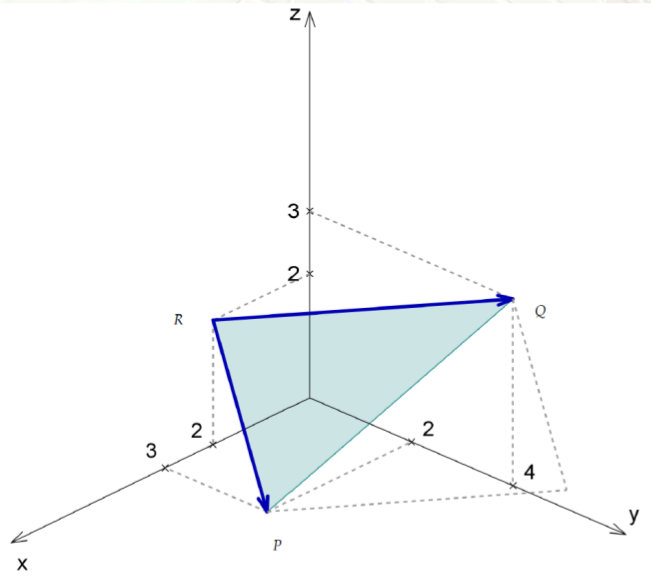
\includegraphics[scale=0.22]{vetor5.png}}\\
    \footnotesize{Fonte:~slides do material da disciplina}
  \end{center}
\end{figure}

\question
Já sabemos que o resultado do produto vetorial entre dois vetores é um
terceiro vetor que é ortogonal aos outros dois. Como podemos
determinar a direção do vetor resultante de um produto vetorial?
\treslinhas

\question
Encontre \vetor{u} tal que $\norm{\vetor{u}} = 3\sqrt{3}$, sendo
\vetor{u} ortogonal ao vetor $\vetor{v} = (2, 3, -1)$ e ao vetor $\vetor{w} =
(2, -4, 6)$. Dos vetores \vetor{u} encontrados, qual deles forma um ângulo
agudo com o vetor $\vetori = (1, 0, 0)$?

\question
Dados os vetores $\vetor{u} = (1, -1, 1)$ e $\vetor{v} = (2, -3, 4)$,
calcular:
\begin{parts}
  \part A área do paralelogramo determinado por \vetor{u} e \vetor{v}.
  \part A altura do paralelogramo relativa à base definida pelo vetor
  \vetor{u}.
\end{parts}

\question
Eu entendi como realizar o produto vetorial entre dois vetores, e
também entendi a relação do produto vetorial com a área do
paralelogramo determinado por esses dois vetores.\\
\begin{oneparcheckboxes}
  \choice Sim
  \choice Não
\end{oneparcheckboxes}


%%%%%%%%%%%%%%%%%%%%%%%%%%%%%%%%%%%%%%%%%%%%%%%%%%%%%%%%%%%%%%%%%%%%%%%%%%%%%%%%%
%%%%%%%%%%%%%%%%%%%%%%%%%%%%%%%%%%%%%%%%%%%%%%%%%%%%%%%%%%%%%%%%%%%%%%%%%%%%%%%%%
%%%%%%%%%%%%%%%%%%%%%%%%%%%%%%%%%%%%%%%%%%%%%%%%%%%%%%%%%%%%%%%%%%%%%%%%%%%%%%%%%
\fullwidth{\section{Produto misto e o cálculo de volumes}}

\question
Sejam três vetores \vetor{u}, \vetor{v} e \vetor{w}. Chamamos de
\emph{produto misto} os 
resultados dos cálculos com a forma $(\vetor{u} \times \vetor{v})
\bigcdot \vetor{w}$. Por que o produto misto é importante?
\treslinhas

\question
Considere a figura abaixo, que ilustra o produto misto $(\vetor{v} \times \vetor{w})
\bigcdot \vetor{u}$:
\begin{figure}[H]
  \begin{center}
    \fbox{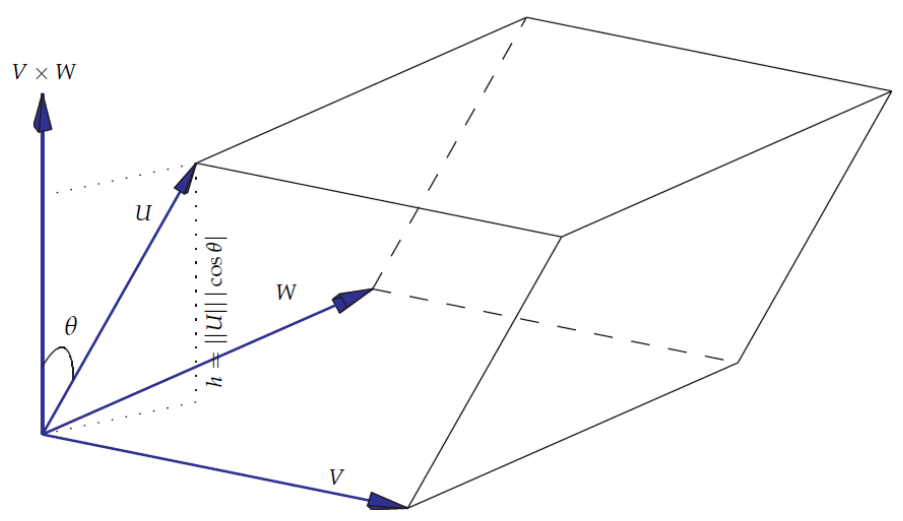
\includegraphics[scale=0.3]{vetor6.png}}\\
    \footnotesize{Fonte:~slides do material da disciplina}
  \end{center}
\end{figure}
\vspace{-0.7cm}
Qual a relação do produto misto com o volume do paralelogramo formado
pelos três vetores utilizados no cálculo?
\duaslinhas

\question
Como calcular o produto misto $(\vetor{v} \times \vetor{w})
\bigcdot \vetor{u}$ com o uso de determinantes?

\question
Por que podemos utilizar o produto misto entre 3 vetores para
determinar se eles estão no mesmo plano?
\treslinhas

\question
Considere os vetores $\vetor{v} = (4, 0, 0)$, $\vetor{w} = (2, 5, 0)$
e $\vetor{u} = (3, 3, 4)$, conforme a figura abaixo:
\begin{figure}[H]
  \begin{center}
    \fbox{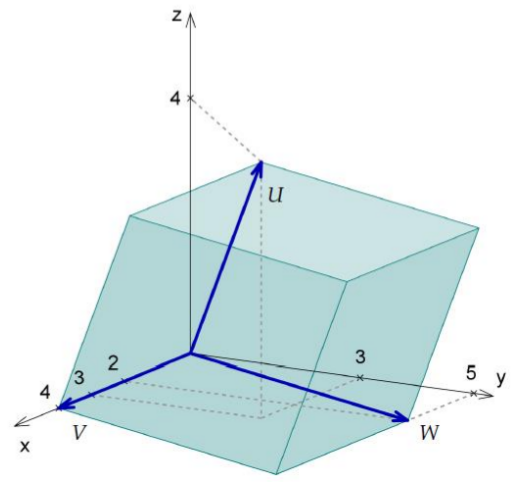
\includegraphics[scale=0.45]{vetor7.png}}\\
    \footnotesize{Fonte:~slides do material da disciplina}
  \end{center}
\end{figure}
\begin{parts}
  \part Calcule o volume do paralelogramo delimitado por esses
  vetores.
  \part Calcule a altura do paralelogramo.
\end{parts}

\question
Qual é o valor de $x$ para que os vetores $\vetor{a} = (3, -x, -2)$,
$\vetor{b} = (3, 2, x)$ e $\vetor{c} = (1, -3, 1)$ sejam
\emph{coplanares}?

\question
Sejam os vetores $\vetor{u} = (1, 1, 0)$, $\vetor{v} = (2, 0, 1)$,
$\vetor{w_1} = (3\,\vetor{u} - 2\,\vetor{v})$, $\vetor{w_2} =
(\vetor{u} + 3\,\vetor{v})$ e finalmente o $\vetor{w_3} = \vetori + \vetorj -
2\,\vetork$. Determinar:
\begin{parts}
  \part O volume do paralelogramo definido por \vetor{w_1},
  \vetor{w_2} e \vetor{w_3}.
  \part A altura do paralelogramo.
\end{parts}

\question
Eu entendi o que é o produto misto entre três vetores e a relação do
produto misto com o volume do paralelogramo formado por esses mesmos
vetores. Também aprendi a determinar se três vetores são coplanares.
\begin{checkboxes}
  \choice Sim
  \choice Não
\end{checkboxes}


\newpage
%%%%%%%%%%%%%%%%%%%%%%%%%%%%%%%%%%%%%%%%%%%%%%%%%%%%%%%%%%%%%%%%%%%%%%%%%%%%%%%%%
%%%%%%%%%%%%%%%%%%%%%%%%%%%%%%%%%%%%%%%%%%%%%%%%%%%%%%%%%%%%%%%%%%%%%%%%%%%%%%%%%
%%%%%%%%%%%%%%%%%%%%%%%%%%%%%%%%%%%%%%%%%%%%%%%%%%%%%%%%%%%%%%%%%%%%%%%%%%%%%%%%%
\fullwidth{\section{Concluindo}}

\question
Estou compreendendo os \emph{conceitos} importantes a respeito de
vetores, e sei \emph{aplicar} e \emph{calcular} diversas coisas com os
vetores.
\begin{checkboxes}
  \choice Sim
  \choice Não
\end{checkboxes}

\question
Estou pronto para a próxima matéria, \emph{Geometria Analítica}!
\begin{checkboxes}
  \choice Sim
  \choice Não
\end{checkboxes}



%%%%%%%%%%%%%%%%%%%%%%%%%%%%%%%%%%%%%%%%%%%%%%%%%%%%%%%%%%%%%%%%%%%%%%%%%%%%%%%%%
%%%%%%%%%%%%%%%%%%%%%%%%%%%%%%%%%%%%%%%%%%%%%%%%%%%%%%%%%%%%%%%%%%%%%%%%%%%%%%%%%
%%%%%%%%%%%%%%%%%%%%%%%%%%%%%%%%%%%%%%%%%%%%%%%%%%%%%%%%%%%%%%%%%%%%%%%%%%%%%%%%%
%%%%%%%%%%%%%%%%%%%%%%%%%%%%%%%%%%%%%%%%%%%%%%%%%%%%%%%%%%%%%%%%%%%%%%%%%%%%%%%%%
%%%%%%%%%%%%%%%%%%%%%%%%%%%%%% TERMINA O DOCUMENTO %%%%%%%%%%%%%%%%%%%%%%%%%%%%%%
%%%%%%%%%%%%%%%%%%%%%%%%%%%%%%%%%%%%%%%%%%%%%%%%%%%%%%%%%%%%%%%%%%%%%%%%%%%%%%%%%
%%%%%%%%%%%%%%%%%%%%%%%%%%%%%%%%%%%%%%%%%%%%%%%%%%%%%%%%%%%%%%%%%%%%%%%%%%%%%%%%%
%%%%%%%%%%%%%%%%%%%%%%%%%%%%%%%%%%%%%%%%%%%%%%%%%%%%%%%%%%%%%%%%%%%%%%%%%%%%%%%%%
%%%%%%%%%%%%%%%%%%%%%%%%%%%%%%%%%%%%%%%%%%%%%%%%%%%%%%%%%%%%%%%%%%%%%%%%%%%%%%%%%
\end{questions}
\end{document}
